
\phantomsection
\addcontentsline{toc}{section}{\textsl{Blåstjernehav Familie- \& Dukketeater}}

{\LARGE \textsl{\textbf{BLÅSTJERNEHAV \\ \\ FAMILIE- \& DUKKETEATER}}}

\label{psh}

\vspace{\fill}

{\Large \textbf{Presentation}}

\bigskip
\bigskip

The project \textsl{Blåstjernehav Familie- \& Dukketeater} proposes two performative modes: 
\begin{enumerate}
\item The play itself -- once a week for instance -- where the kids play in the boat-carrousel with interactive quadrophonic soundscape for their families and audience;
\item and the stage of the play as a fjord-landscape `3D-tableau' installation with experimental sonic sculpture.
\end{enumerate}

\bigskip

The following documentation shows a possible play, and it is best to visualize it as a sketch, showing how the theatre was played and exhibited in Tromsø Kunstforening from 14th of August to 11th of October 2020. 

\bigskip

\begin{figure}[h]
		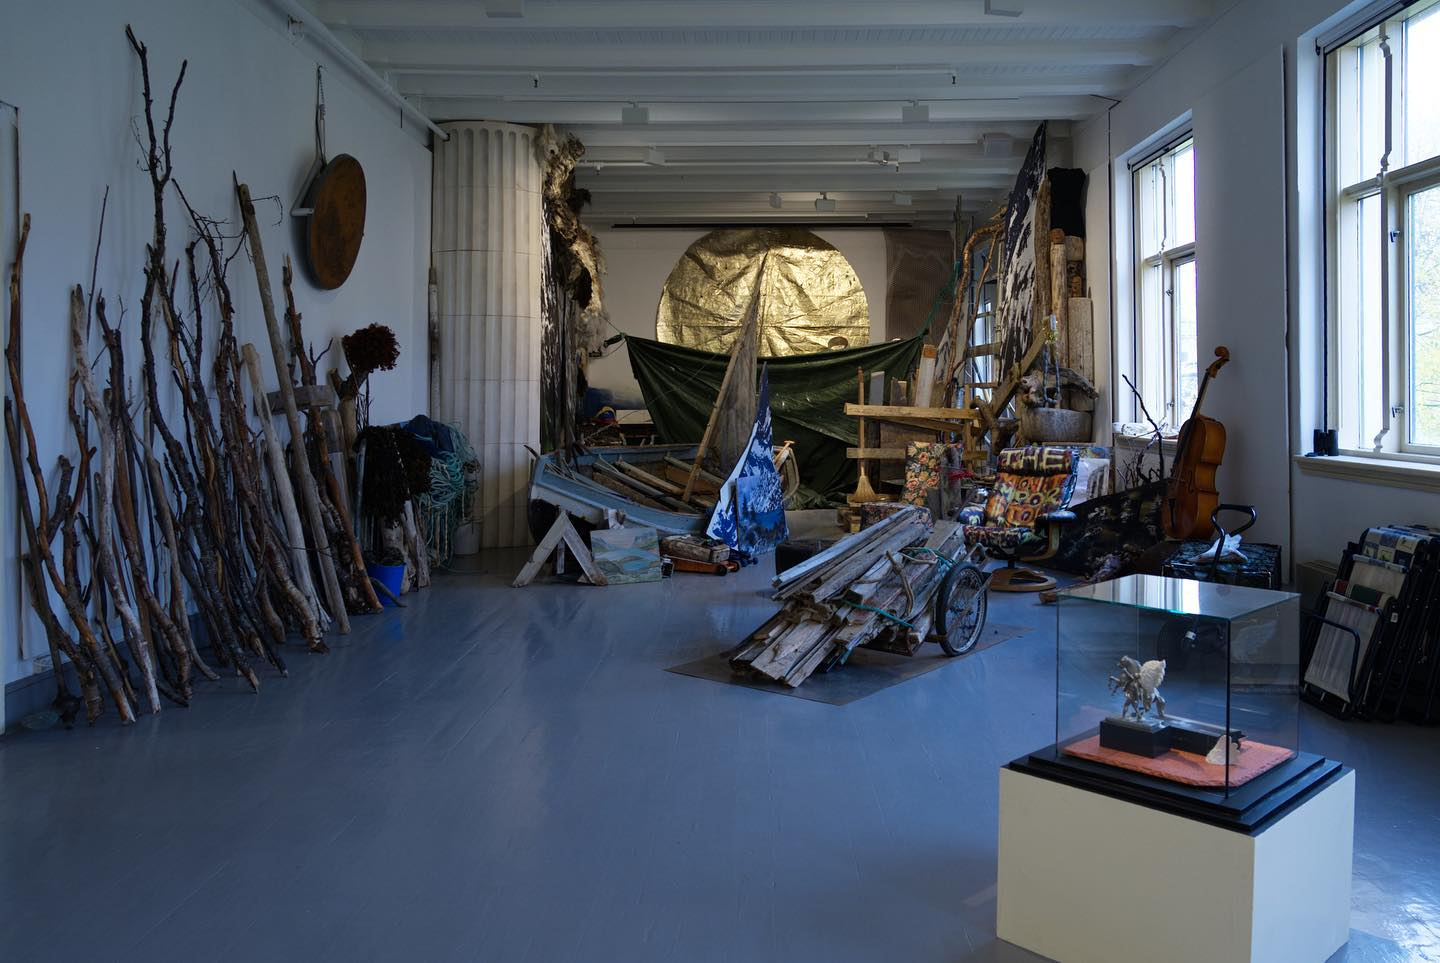
\includegraphics[width=\textwidth]{mp/img/img1}
		%\caption{}
		\label{sh}
\end{figure}

\newpage 

{\Large \textsl{\textbf{Selenes Havbrev}}}

\bigskip

\noindent \textbf{\textsl{Ly til fantasi og fellesskap}} 14.08.2020 -- 11.10.2020 \vspace{1mm} \\ 
$\rightarrow$ \href{http://www.tromsokunstforening.no/default.asp?cmd=100&UtsID=200}{\texttt{\footnotesize http://www.tromsokunstforening.no/Ly\_til\_fantasi\_og\_fellesskap}} 

\bigskip

[ ... ] \textsl{Forestillingen 'Selenes havbrev' og 'Selenes sang' er skrevet av Ane Elene Johansen, og maleriene er laget av Asbjørn Hillingseter Løyning. Yann Ics har komponert musikk og lydbilde, og scenografien er laget av Håvard Arnhoff som også er initiativtakeren bak teateret.}

\smallskip

\begin{figure}[h]
	\begin{center}
		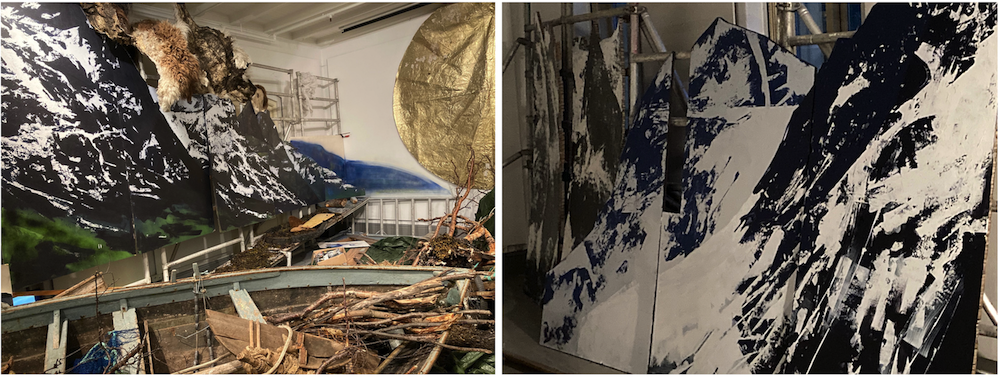
\includegraphics[width=0.99\textwidth]{mp/img/img2}
		%\caption{}
		\label{sh}
	\end{center}
\end{figure}

\begin{enumerate}
\item \textbf{The play} $\rightarrow$ pages \pageref{shtp1} to \pageref{shtp2}. 
\begin{figure}[H]
\hfill 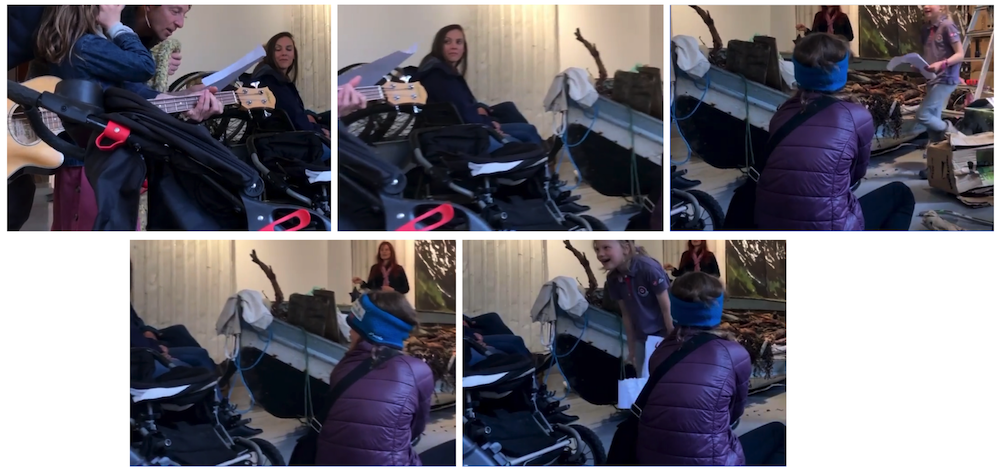
\includegraphics[width=0.92\textwidth]{mp/img/img3}
\end{figure} 
\item \textbf{On the side} \\ \\ 
$\rightarrow$ Study of a sonic sculpture on two recycled corrugated sheets as installation from the 22nd of August to the 29th of August 2020 in Tromsø Kunstforening.
\begin{figure}[H]
\hfill 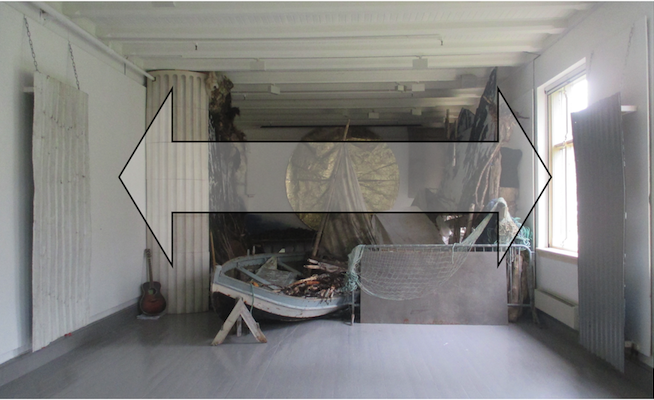
\includegraphics[width=0.92\textwidth]{mp/img/img4}
\end{figure}
This installation performed the score of the second guitar of the composition \textsl{Selenes Havbrev} [ $\rightarrow$ page \pageref{sh} ] with the digital wave guide physical model of a bowed instrument plus improvised composition. \\ \\
$\rightarrow$ Surrealistic sound installation performed in Tromsø Kunstforening between the 25th of September and the 11th of October 2020. 
\begin{figure}[H]
\hfill 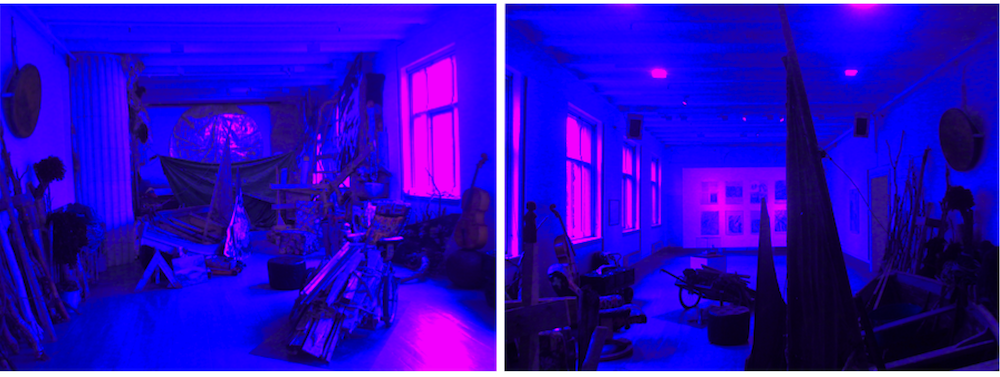
\includegraphics[width=0.92\textwidth]{mp/img/img5}
\end{figure}
Experimenting different physical models -- as a bowed instrument and the acoustics of tube models -- using respectively a cello and on a parabolic antenna, as part of a `post-apocalyptic' ambient quadraphonic soundscape which the latest can be depicted as a  `walking on the \textit{Ersfjordbotn} beach'.
\end{enumerate}

\begin{figure}[htp]
	\begin{center}
		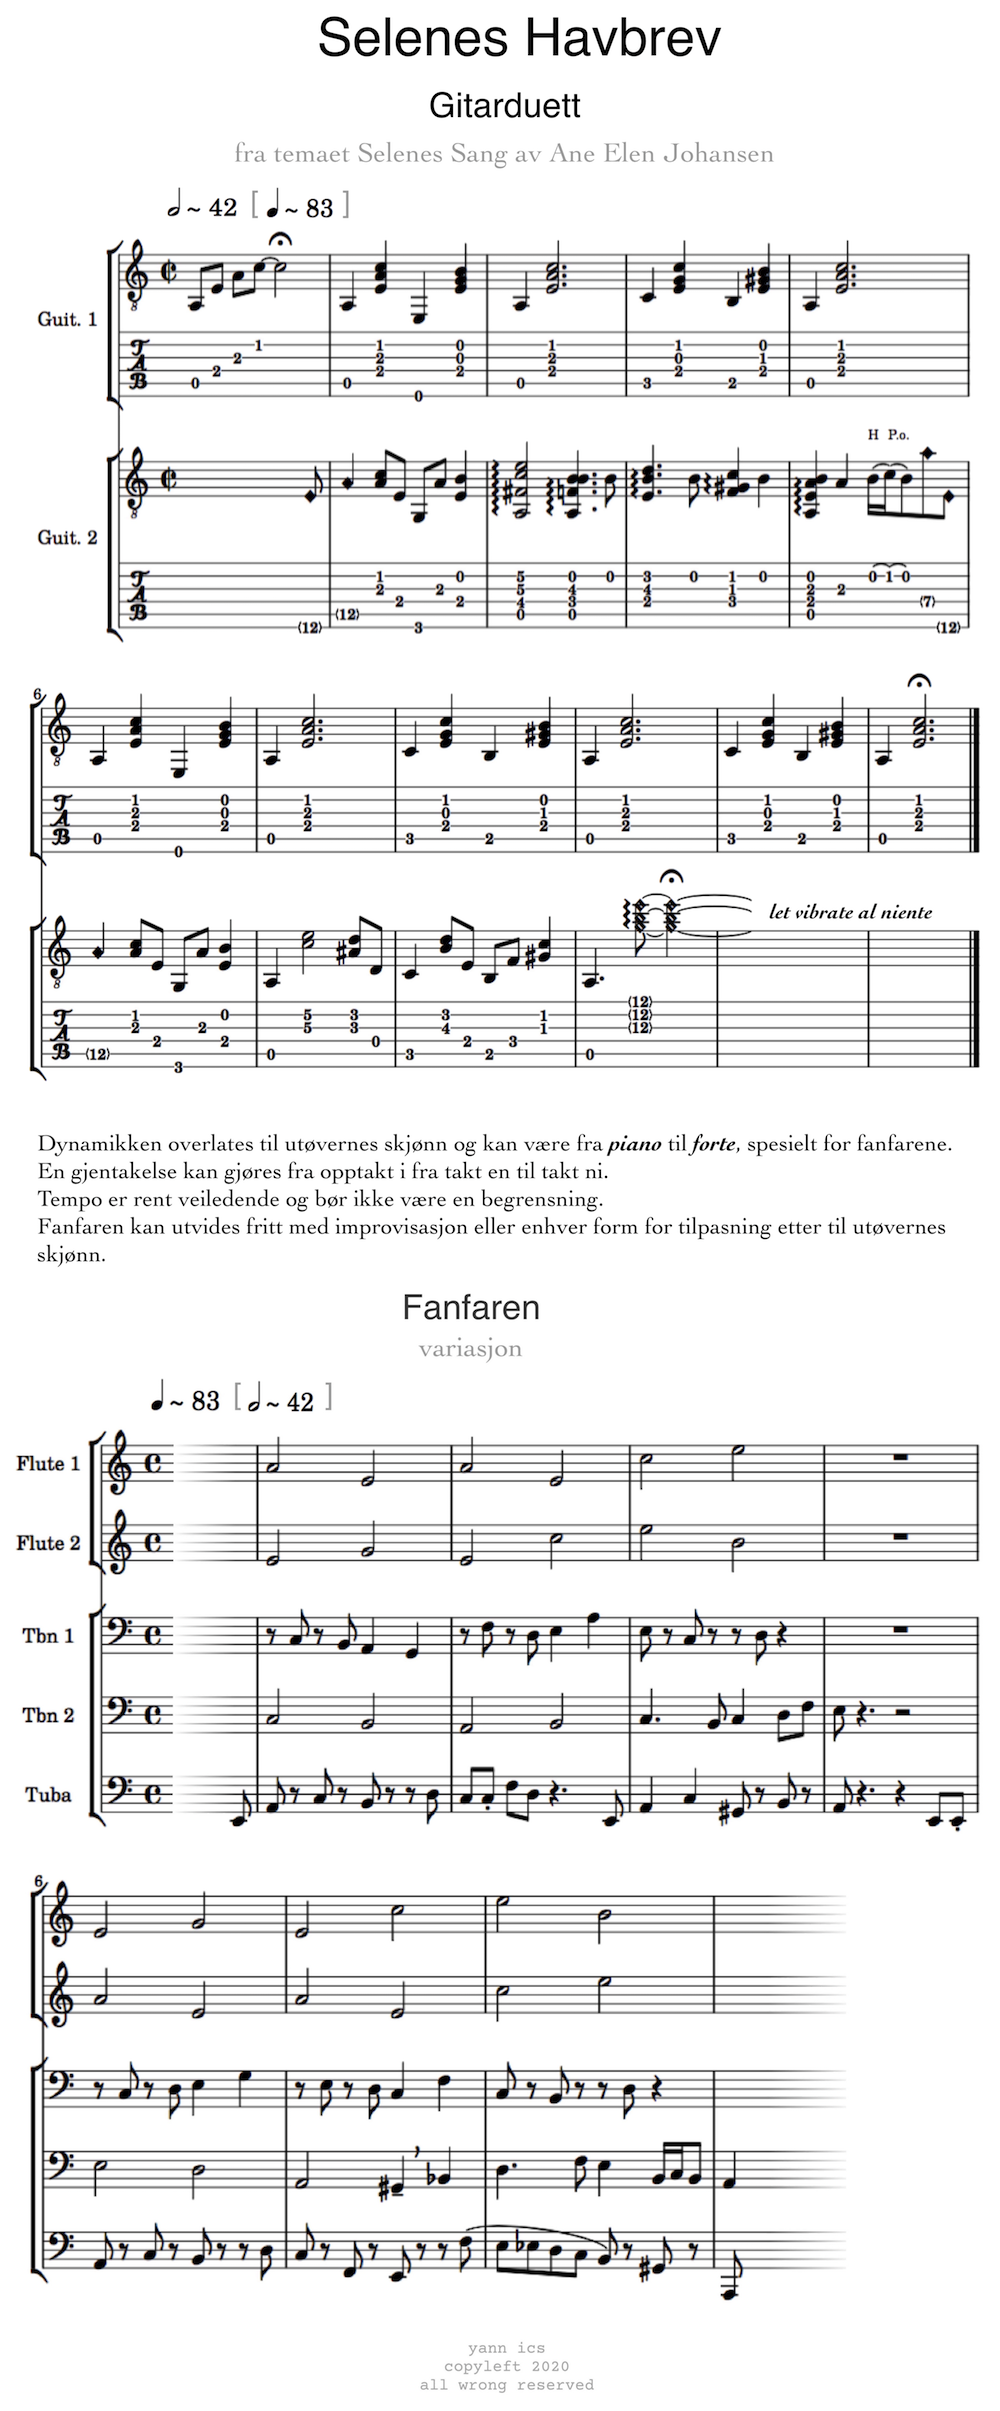
\includegraphics[width=0.65\textwidth]{mp/img/img6}
		%\caption{}
		\label{sh}
	\end{center}
\end{figure}

\bigskip
\bigskip
\bigskip
\bigskip

\label{shtp1}

\begin{center}
  \LARGE\bfseries{\textsl{Selenes Havbrev}}
\end{center}

\bigskip
\bigskip
{\small 
\hfill \textbf{av Ane E. Johansen.}

\bigskip 
 \bigskip

\noindent \textit{\color{gray} En fjord. Fjære. En båt.}

\noindent \textit{\color{gray} Ei jente kjem fram av båten. Kravlende ut, som ei forsiktig krabbe. Stiller seg fram på scenen og proklamerer:}

\begin{description}
\item[Marikkel]: I natt hadde æ en drøm. Tre lysende stjerner så vi på vårsolas himmel i natt. Det betyr at selene kjem med Havbrevet. Æ og mi søster skal stå klar og ta imot! 
\item[Sardina]: Han pappa sover inne i huset enda. Han treng søvnen sin no, for ho mamma har kommet til himmelen og han pappa er fryktelig lei seg.
\end{description}

\noindent \textit{\color{gray} Samtidig som Sardina sier dette, går Marikkel og setter seg i båten og venter. Hun tar på seg en sydvest og begynner å ordne til noe fiskesaker.}

\noindent \textit{\color{gray} Sola glinser i horisonten. Lyset er vidunderlig. Det skinner på fjellsidene.}

\begin{description}
\item[Sardina]: Marikkel, har du sjekka nisa om den e klar?
\item[Marikkel]: Jada, vi har alt på stell. Trur du vi ska fare med én gang?
\item[Sardina]: Best å ikkje vente for lenge. Æ drømte at vi måtte være klar på stiganes flo!
\item[Marikkel]: Tenk at vi har drømt det samme! Men med floa kjem vinden..
\item[Sardina]: Det e no eller aldri!
\end{description}

\noindent \textit{\color{gray} Sardina skyver båten ut mot vannet og hiver seg oppi båten. De tar fram årene og begynner å ro. De ror og ror seg lengre og lengre utover fjorden. Med ett blåser det opp til storm.}

\begin{description}
\item[Marikkel]: Det blåser opp til storm! Vi må snu! 
\end{description}

\noindent \textit{\color{gray} De får vansker med å holde årene, og de mister ei åre i bølgene.}

\begin{description}
\item[Sardina]: Å nei, jeg mista åra! Hjelp meg, får du tak i den? 
\item[Marikkel]: Nei, den forsvinner!
\end{description}

\noindent \textit{\color{gray} Sardina bøyer seg over ripa og prøver å få tak i den, og plutselig faller hun ned i vannet.}

\begin{description}
\item[Sardina]:  \textit{\color{gray} (roper)} Marikkel! 
\end{description}

\noindent \textit{\color{gray} Uværet fortsetter, og Sardina holder på å drukne. Marikkel forsøker å nå henne med den ene åra si. Sardina forsvinner lengre og lengre bort fra båten. Marikkel ror etter og prøver å nå henne igjen. Men det er sterke bølger og hardt å ro.}

\begin{description}
\item[Marikkel]: Ta åra! Ta åra!
\end{description}

\noindent \textit{\color{gray} Sardina griper i panikk rundt åra og Marikkel greier å få henne om bord i båten igjen. Sardina klemmer i ett hardt grep rundt Marikkel og da hoster Marikkel og våkner til liv.}

\begin{description}
\item[Sardina]:  \textit{\color{gray} (hoster)} Hvor kom det uværet fra? 
\item[Marikkel]: Flovinden, Sardina! Æ sa det til dæ! Vi må bare fortsette å ro. Vi er kommet så langt no, vi vil ikkje klare å ro mot bølgan inn til land igjen. 
\end{description}

\noindent \textit{\color{gray} De ror med årene som er igjen gjennom uværet.}

\begin{description}
\item[Marikkel]: Her kan vi gå i land! 
\end{description}

\noindent \textit{\color{gray} De ror seg i land ved ei bukt og drar båten i land og fortøyer den. Sakte gir uværet seg og det blir blank stilla hav.}

\begin{description}
\item[Sardina]: Se, Marikkel!  \textit{\color{gray} (Peker på himmelen)} Tre stjerner på vårsolas himmel. Det var hit vi skulle, uværet ledet oss hit!
\item[Marikkel]: Ja, tenk at det blei sånn!
\item[Marikkel]: Da er tida inne.  \textit{\color{gray} (En liten pause til ettertanke)} 
\end{description}

\noindent \textit{\color{gray} Sola lyser fram igjen og det glitrende landskapet trer fram i lyset.}

\noindent \textit{\color{gray} Plutselig hører de noe i havet som fanger oppmerksomheten deres. Tre seler kjem svømmende mot dem.}

\begin{description}
\item[Sardina]: Der kjem selene  \textit{\color{gray} (sier det andektig)}. 
\end{description}

\noindent \textit{\color{gray} Selene holder et tau i munnene sine. Den ene til den andre. Tauet er spunnet av tang. I tauet henger det ei lita kiste. Selene kjem i land i fjærsteiene og danser på sitt fornurlige vis mot jentene. Selene synger:}

\begin{description}
\item[Selene]: \textit{\color{gray} (Selenes Sang)} 
\end{description}

\begin{quote}
\begin{guitar}
\smallskip
I [\color{gray} Am]natt har vi [\color{gray} Em]spunnet ei vi[\color{gray} Am]se\smallskip
Tre [\color{gray} C]stjerner i vår[\color{gray} E]solelyset[\color{gray} Am]\smallskip
Vårt [\color{gray} Am]brev kjem fra ha[\color{gray} Em]vets kiste[\color{gray} Am]\smallskip
[\color{gray} C]Aldri må vi glem[\color{gray} E]me eller miste.[\color{gray} Am]

\end{guitar}
\end{quote}

\noindent \textit{\color{gray} Selene gir kista til jentene. Jentene takker og bukker.} 

\begin{description}
\item[Marikkel]: Takk skal dere ha. 
\item[Sardina]: Hvordan kan en drøm bli sann? 
\item[Selene]: \textit{\color{gray} (sier i kor)} Drømte dere hva dere skulle gjøre med brevet vi har kommet med? 
\item[Marikkel]: \textit{\color{gray} (Forundret)} Nei, her stopper drømmen. 
\end{description}

\noindent \textit{\color{gray} Jentene ser på hverandre.}

\begin{description}
\item[Selene]: \textit{\color{gray} (sier i kor)} Aldri må vi glemme eller miste, drømmen om blåstjernehav. Ta dette brevet og gi det til den dere holder mest av. 
\end{description}

\noindent \textit{\color{gray} Så forsvinner selene ut i havets dyp.}

\noindent \textit{\color{gray} Jentene står igjen med den lille kista.} 

\begin{description}
\item[Marikkel]: Hva mente selene? Aldri må vi glemme eller miste, drømmen om blåstjernehav. Ta dette brevet og gi det til den dere holder mest av \textit{\color{gray} (repeterer etter selene)}. 
\item[Sardina]: Nei, si det. Kanskje vi må gi det til den vi stoler mest på i hele verden? 
\end{description}

\noindent \textit{\color{gray} De åpner kista. Der ligger det et blått hjerte av glass. Marikkel tar hjertet varsomt ut av kista og holder det opp mot lyset.}

\begin{description}
\item[Marikkel]: Se, kor vakkert!
\item[Sardina]: Ja, se kor det glinse og banke! Et blått hjerte!
\end{description}

\noindent \textit{\color{gray} De studerer hjertet. Ser det fra alle vinkler, beundrer det.}

\begin{description}
\item[Marikkel]: Vi tar det med hjem til han pappa, så blir han glad.
\item[Sardina]: Ja, det gjør vi!
\end{description}

\noindent \textit{\color{gray} De hiver seg i båten, men oppdager at den begynner å ta inn vatn.}

\begin{description}
\item[Marikkel]: Se, søster, båten begynner å ta inn vann!
\item[Sardina]: Vi kan ikkje komme oss hjem over fjellene!
\end{description}

\noindent \textit{\color{gray} De ser seg omkring på fjellene rundt. Og stirrer ut i havet.}

\begin{description}
\item[Marikkel]: \textit{\color{gray} (Sier rolig og bestemt)} Da er vi nødt til å ro hjem. 
\end{description}

\noindent \textit{\color{gray} De setter båten i havet og begynner å ro. Et alvor legger seg over stemninga. De skjønner at dette kommer til å bli farlig.} 

\begin{description}
\item[Sardina]: Vi får ro så stødig og fort vi bare kan. 
\end{description}

\noindent \textit{\color{gray} De kommer inn i en god rytme. Nå og da tar Marikkel øsekaret og hiver ut vann fra båten. De ror og de ror. Jo lengre de ror, jo mer må de bruke øsekaret. De ser bakover for å se hvor langt de har igjen.}

\begin{description}
\item[Marikkel]: Å, no må det ikkje være langt igjen! Båten tar inn mer og mere vann! 
\item[Sardina]: Vi må bare holde ut! Æ håpe vi rekk det!
\item[Marikkel]: \textit{\color{gray} (ser seg bakover og studerer huset og naustet der de bor)} E det ikkje han pappa som står i fjærsteinan der borte?
\item[Sardina]: Jo, det e det! Pappa!
\end{description}

\noindent \textit{\color{gray} Mannen i fjæra vinker med begge armene, og roper tilbake.}

\begin{description}
\item[Pappa]: Sardina og Marikkel!
\end{description}

\noindent \textit{\color{gray} Mannen hiver seg i en båt og ror i møte med dem. Når båtene møtes, klyver Sardina og Marikkel i pappas båt, og han fortøyer den fast i sin egen.}

\begin{description}
\item[Sardina og Marikkel]: Pappa! 
\end{description}

\noindent \textit{\color{gray} De gir hverandre en stor klem.}

\begin{description}
\item[Pappa]: Jentene mine. E dokker ute på havet no, med den gamle båten! Den læk, jo! Og så tidlig på morran mens æ søv. Nei og nei, æ har vært så redd førr kor dokker va! 
\item[Marikkel]: Pappa, vi, unnskyld! Vi hadde en drøm om at vi måtte på havet, og så fikk vi ikkje sove. Pappa, vi –
\item[Sardina]: \textit{\color{gray} (avbryter)} Pappa, vi har opplevd så mye! Vi har møtt sela og, vi mesta ei åra, det va så mye bølga, og selan ga oss nokka vi ville gje tel dæ-
\item[Pappa]: Har selan gjedd dokker nokka, nei, ka dokker førtell- 
\item[Marikkel og Sardina]: \textit{\color{gray} (i kor, andektig)} Aldri må vi glemme eller miste, drømmen om blåstjernehav. Ta dette brevet og gi det til den dere holder mest av. 
\end{description}

\noindent \textit{\color{gray} Sardina og Marikkel åpner kista av skjell og gir det blå hjertet til pappa.}

\begin{description}
\item[Pappa]: \textit{\color{gray} (utbryter)} Åh….! Mammas gamle smykkestein! Kordan…?
\end{description}

\noindent \textit{\color{gray} Pappa holder det varsomt og stryker det blå hjertet forsiktig. Tårene renner nedover kinnene hans.}

\begin{description}
\item[Marikkel]: E det mamma sin smykkestein- ! 
\end{description}

\noindent \textit{\color{gray} Marikkel og Sardina ser på hverandre. De alle ser på hverandre spørrende.} 

\noindent \textit{\color{gray} Med ett hører de en fanfare i horisonten. Det er melodien som selene sang. De klemmer hverandre og smiler. Lyset gnistrer og blender.}
\color{black}
\label{shtp2}}

\bigskip
\bigskip
\bigskip 

\begin{figure}[h!]
	\begin{center}
		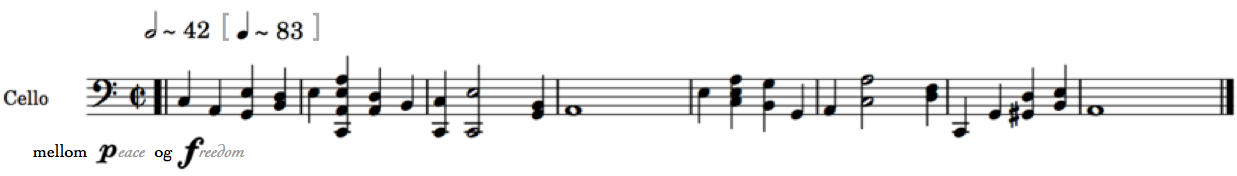
\includegraphics[width=1\textwidth]{mp/img/img7}
		%\caption{}
		\label{ps}
	\end{center}
\end{figure}
